% =========================================================================== %

\begin{frame}[t,plain]
\titlepage
\end{frame}

% =========================================================================== %

\begin{frame}{Recap}
%
\begin{columns}[T]
\column{.5\linewidth}
\begin{itemize}
\item Vocabulary
	\begin{itemize}
	\item Terminal
	\item Interpreter
	\item IDE
	\end{itemize}
\item Terminal
	\begin{itemize}
	\item Text-based commands with parameters
	\item CWD (current working directory)
	\item Invoking the Python interpreter
	\end{itemize}
\item Comments
	\begin{itemize}
	\item Pound-Symbol (\texttt{\#}) begins a comment
	\item The entire line behind is ignored
	\end{itemize}
\end{itemize}
%
\column{.5\linewidth}
\begin{itemize}
\item Command \inPy{print}
	\begin{itemize}
	\item Output of text on screen
	\item Parameters (aka arguments) in parenthesis, separated by commas
	\item Texts in quotes ('single' or ''double'')
	\end{itemize}
\item Variables
	\begin{itemize}
	\item Memory cells with changeable content
	\item Symbol and associated data type
	\item Computing and updating values
	\item Can be used with \inPy{print}
	\end{itemize}
\end{itemize}
\end{columns}
%
\begin{center}
	\emph{Any Questions?}
\end{center}
%
\end{frame}

% =========================================================================== %

\begin{frame}{Recap}
%
\begin{columns}[T]
\column{.5\linewidth}
\begin{itemize}
\item Converting Data Types
	\begin{itemize}
	\item Use the name of the data type as a function, \zB \inPy{int("3")}
	\item Possible Loss of information: \\
		\inPy{int(3.1)} ~\thus~ \inPy{3}
	\end{itemize}
\item Format Strings
	\begin{itemize}
	\item \inPy{f"Text {expression:format}"}
	\item number of digits and decimals, alignment, ...
	\item Use literature on demand
	\end{itemize}
\end{itemize}
%
\column{.5\linewidth}
\begin{itemize}
\item Booleans (truth values)
	\begin{itemize}
	\item Type \inPy{bool} stores \inPy{True} or \inPy{False}
	\item Comparison operators (\inPy{==}, \inPy{>=}, ...)
	\end{itemize}
\item Conditional execution of code
	\begin{itemize}
	\item With \inPy{if} and indentations
	\item \inPy{elif}: alternative condition
	\item \inPy{else}: otherwise
	\item Tests conditions from top to bottom
	\item Executes only first hit
	\item Can be nested
	\end{itemize}
\end{itemize}
\end{columns}
%
\begin{center}
	\emph{Any Questions?}
\end{center}
%
\end{frame}

% =========================================================================== %

\begin{frame}[fragile]{Seen in the Exercises}
%
\begin{itemize}
\item Quotes in a string
	\begin{itemize}
	\item Easiest solution: \emph{Escape Character} \texttt{\textbackslash}:
		\begin{itemize}
		\item \inPy{stringVar = "\"That's a pity\", she said."}
		\item \emph{Escape Character}: Character that tells python that the following character is to be interpreted in a different manner
		\item Examples: \inPy{"\n"} -- newline (line break); \inPy{"\t"} -- tabulator, \inPy{"\\"} -- backslash
		\end{itemize}
	\item Alternative: \emph{String Concatenation} with single and double quotes
		\begin{itemize}
		\item \inPy{stringVar = '"That' + "'s a pity" + '", she said."}
		\end{itemize}
	\end{itemize}
\end{itemize}
%
\end{frame}

% =========================================================================== %

\begin{frame}[fragile]{Question asked in an exercise}
%
\begin{center}
	\begin{Large}
	\emph{Is it possible to enter equations and let Python evaluate them?}
	\end{Large}
\end{center}
%
\begin{itemize}
\item Jes, but this is dangerous.
\item (There are safe, but \emph{very} complicated alternatives.)
\item Command \inPy{eval} takes a string argument and runs it as Python code.
\item Returns result of this evaluation: \inPy{result = eval("x** 2 + 5")}
\item String may contain \emph{arbitrary} Python code -- including harmful commands!
\end{itemize}
%
\begin{warnbox}[Code Injection und \texttt{eval}]
User input is \emph{always} a potential source of harm, even without malicious intent. They should \emph{always} be tested to be in the range of acceptable values (\Thus \inPy{if}) and limited as much as possible.
\end{warnbox}
%
\end{frame}

% =========================================================================== %

\begin{frame}{xkcd: Exploits of a Mom}
%
\begin{center}
	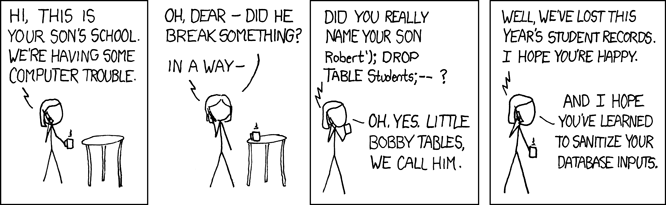
\includegraphics[width=.8\linewidth]{./gfx/xkcd-codeInjection}\\
	\vspace{3pt}
	
	\scriptsize \emph{Her daughter is named Help I'm trapped in a driver's license factory.}
	\vspace{6pt}\\
	
	Source: \url{https://xkcd.com/327/}
\end{center}
%
\end{frame}

% =========================================================================== %

\begin{frame}{Chapter 3}
%
\begin{itemize}
\item Modules
	\begin{itemize}
	\item Collections of Routines
	\item Load to use pre-written functions
	\end{itemize}
\end{itemize}
%
\end{frame}

% =========================================================================== %

\begin{frame}[fragile]
%
\begin{columns}
\column{.5\linewidth}
\begin{Large}
Loading Modules
\vspace{6pt}
\end{Large}
\begin{itemize}
\item Python only has 33 keywords
\item From these it is possible to construct \enquote{complex machinery}
\item Requires time and memory to load
\item Never necessary to use all of them at once
\item[\Thus] Load \enquote{on demand}
\item[\Thus] Command \inPy{import}
\item Module: Collection of pre-built solutions
\end{itemize}
%
\column{.5\linewidth}
\begin{codebox}[Syntax: \texttt{import}]
\begin{minted}[fontsize=\scriptsize]{python}
import modulename
\end{minted}
\end{codebox}
\begin{itemize}
\item Example: \texttt{math}: common mathematical funvctions (exp, sin, sqrt, ...)
\item Example: \texttt{cmath}: same funcitons for complex numbers
\item Loads code into memory
\item Code is from...
	\begin{itemize}
	\item either: CWD
	\item or: some standard directory
	\end{itemize}
\end{itemize}
\end{columns}
%
\end{frame}

% =========================================================================== %

\begin{frame}[fragile]{Using Functions from Modules}
%
\begin{columns}
\column{.5\linewidth}
\begin{itemize}
\item Two Modules can each hold a function of the same name
\item Hence: \inPy{modulename.object}
\item Object: function or constant (or other constructs)
\end{itemize}
%
\column{.5\linewidth}
\begin{itemize}
\item \texttt{sin} -- Sine
\item \texttt{pi} -- $\pi$
\item Both available for real-valued (\texttt{math}) and complex-valued operations (\texttt{cmath})
\end{itemize}
\end{columns}
%
\begin{tcbraster}[raster columns=2,
                  raster equal height,
                  nobeforeafter,
                  raster column skip=0.5cm]
\begin{codebox}[Example: Sine from two modules]
\begin{minted}[fontsize=\scriptsize]{python}
import cmath
import math

print( math. sin( math.pi / 2) )
print( cmath.sin(cmath.pi / 2) )
\end{minted}
\end{codebox}
%
\begin{cmdbox}[Output: Sine from two modules]
\begin{minted}[fontsize=\scriptsize]{text}
1.0
(1+0j)
\end{minted}
\end{cmdbox}
\end{tcbraster}
%
\end{frame}

% =========================================================================== %

\begin{frame}{Chapter 4}
%
\begin{itemize}
\item Data Containers
	\begin{itemize}
	\item Modell of the memory
	\item Mutable vs. Immutable
	\item \inPy{list}s
	\item Slices
	\item Methods and special functions
	\end{itemize}
\end{itemize}
%
\end{frame}

% =========================================================================== %

\begin{frame}[fragile]{Data containers -- \inPy{list}s}
%
\begin{columns}
\column{.5\linewidth}
\begin{itemize}
\item So far: only handle singlular units of information at once (single numbers)
\item We often need \emph{lists} of values
\item New data type: \inPy{list}
\item Composition of arbitrary many values of arbitrary type
\item Acessible via an \emph{index} (think of the \enquote{row of the list})
\item \emph{Indices start at 0!}
\end{itemize}
%
\column{.5\linewidth}
\begin{codebox}[Syntax: Creating \texttt{list}s]
\begin{minted}[fontsize=\scriptsize]{python}
variable = [element1, element2, ...]
\end{minted}
\end{codebox}
%
\begin{codebox}[Syntax: Changig elements in a \texttt{list}]
\begin{minted}[fontsize=\scriptsize]{python}
variable[index] = newValue
\end{minted}
\end{codebox}
%
\begin{codebox}[Syntax: reading \texttt{list} elements]
\begin{minted}[fontsize=\scriptsize]{python}
print( variable[index] )
\end{minted}
\end{codebox}
\end{columns}
%
\end{frame}

% =========================================================================== %

\begin{frame}[fragile]
%
\begin{tcbraster}[raster columns=2,
                  raster equal height,
                  nobeforeafter,
                  raster column skip=0.5cm]
\begin{codebox}[Example: \texttt{list}s]
\begin{minted}[fontsize=\scriptsize, linenos]{python}
values = [1, 2, 3, 
          "other data type", 
          ["a", "list", "within", 
           "the", "list"]
         ]
print(values)
print(values[0])
print(values[4])
\end{minted}
\end{codebox}
%
\begin{cmdbox}[Output: \texttt{list}s]
\begin{minted}[fontsize=\scriptsize]{text}
[1, 2, 3, 'other data type', ['eine', 
 'Liste', 'in', 'der', 'Liste']]
1
['a', 'list', 'within', 'the', 'list']
\end{minted}
\end{cmdbox}
\end{tcbraster}
%
\end{frame}

% =========================================================================== %

\begin{frame}[fragile]
%
\begin{columns}[t]
\column{.45\linewidth}
\begin{Large}
{Indices: Extended Features}
\vspace{6pt}
\end{Large}
\begin{itemize}
\item Negative Indices: \enquote{count back from the end}
	\begin{itemize}
	\item \texttt{variable[-1]}: last element of a \inPy{list}
	\end{itemize}
\item \enquote{Slices}
	\begin{itemize}
	\item Select a subsection of a list
	\item Syntax \enquote{start : stop : stride} \\
		(where all of them are \inPy{int}s)
	\item Parts can be ommitted
	\item \texttt{variable[start:stop]}: everything from index \texttt{start} (inclusive) and up to index \texttt{stop} (exclusive)
	\item \texttt{variable[start::n]}: every n-th, beginning at index \texttt{start}
	\end{itemize}
\end{itemize}
%
\column{.55\linewidth}
\begin{codebox}[Example: Index-Features]
\begin{minted}[fontsize=\scriptsize, linenos]{python}
myList = [0, 1, 2, 3, 4, 5, 6, 7, 8, 9, 10]
print(myList[-1], myList[-2])
print(myList[0:-1:2])
print(myList[2::2])
print(myList[::2])
print(myList[:5])
\end{minted}
\end{codebox}
%
\begin{cmdbox}[Output]
\begin{minted}[fontsize=\scriptsize]{text}
10 9
[0, 2, 4, 6, 8]
[2, 4, 6, 8, 10]
[0, 2, 4, 6, 8, 10]
[0, 1, 2, 3, 4]
\end{minted}
\end{cmdbox}\end{columns}
%
\end{frame}

% =========================================================================== %

\begin{frame}[fragile]{Copying -- Unexpected Effects}
%
\begin{tcbraster}[raster columns=2,
                  raster equal height,
                  nobeforeafter,
                  raster column skip=0.5cm]
\begin{warnbox}[Example: working copy (erroneous), leftupper=7mm]
\begin{minted}[fontsize=\scriptsize, linenos]{python}
myList = [0, 1, 2, 3, 4, 5, 6, 7, 8, 9]
copiedList = myList
myList[0] = "altered"
print(copiedList)
\end{minted}
\end{warnbox}
%
\begin{cmdbox}[Output: working copy (erroneous)]
\begin{minted}[fontsize=\scriptsize]{text}
['altered', 1, 2, 3, 4, 5, 6, 7, 8, 9]
\end{minted}
\end{cmdbox}
\end{tcbraster}
%
\begin{itemize}
\item Expectation: Changing \texttt{myList} should not have any influence on \texttt{copiedList}
\item What's actually going on?
\item[\Thus] \emph{References}
\end{itemize}
%
\end{frame}

% =========================================================================== %

\begin{frame}[fragile]
%
\begin{tcolorbox}[title=Memory Modell]
\begin{center}
\begin{tikzpicture}
  [ 
    cell/.style={text width=8mm,
      text height=4mm, draw=black, inner sep=1mm},
    ld/.style={draw=blue,shorten >=2pt,->}
  ]
  \node (c1) at (0,0) [cell] {\ttfamily 99};
  \node (c2) at (1,0) [cell] {\ttfamily 1};
  \node (c3) at (2,0) [cell] {\ttfamily 255};
  \node (c4) at (3,0) [cell] {\ttfamily 0};
  \node (c5) at (4,0) [cell] {\ttfamily 80};
  \node (c6) at (5,0) [cell] {\ttfamily ...};

  \node (labelMem) at (8,  1) {Symbols in code};
  \node (labelMem) at (8,  0) {Values in memory};
  \node (labelMem) at (8, -1) {Adresses};
  
  \node (a1) [below=2mm of c1]             {\tiny 0x27ff};
  \node (a2) [below=2mm of c2, color=teal] {\tiny 0x2800};
  \node (a3) [below=2mm of c3]             {\tiny 0x2801};
  \node (a4) [below=2mm of c4]             {\tiny 0x2802};
  \node (a5) [below=2mm of c5]             {\tiny 0x2803};
  \node (a6) [below=2mm of c6]             {\tiny 0x2804};
  
  \node (ptr) [below=8mm of c1] {\scriptsize Adresse von \texttt{x}};
  \node (vc2) [above=6mm of c1] {\scriptsize Variable \texttt{x}};
  \node (vc0) [above=2mm of c1] {\scriptsize Variable \texttt{y}};
  
  \draw [ld, teal] (ptr.east) .. controls +(0.3,0) .. (a2.south);
  \draw [ld]       (vc0.east) .. controls +(0.4,0) .. (c2.north);
  \draw [ld]       (vc2.east) .. controls +(2.4,0) .. (c4.north);
\end{tikzpicture}
\end{center}
\end{tcolorbox}
%
\begin{itemize}
\item Variables really only store \emph{adresses}
\item Access to referenced memory cells
\end{itemize}
%
\end{frame}

% =========================================================================== %

\begin{frame}[fragile]
%
\begin{tcolorbox}[title={\footnotesize Memory modell -- What we want}]
\begin{center}
\begin{tikzpicture}
  [ 
    cell/.style={text width=8mm,
      text height=4mm, draw=black, inner sep=1mm},
    ld/.style={draw=blue,shorten >=2pt,->}
  ]
  \node (gap1) at ( 0,0)        {\ttfamily ...};
  \node (v1)   at ( 1,0) [cell] {\ttfamily 1};
  \node (v2)   at ( 2,0) [cell] {\ttfamily 2};
  \node (v3)   at ( 3,0) [cell] {\ttfamily 3};
  \node (v4)   at ( 4,0) [cell] {\ttfamily 4};
  \node (gap2) at ( 5,0)        {\ttfamily ...};
  \node (c1)   at ( 6,0) [cell] {\ttfamily 1};
  \node (c2)   at ( 7,0) [cell] {\ttfamily 2};
  \node (c3)   at ( 8,0) [cell] {\ttfamily 3};
  \node (c4)   at ( 9,0) [cell] {\ttfamily 4};
  \node (gap3) at (10,0)        {\ttfamily ...};
  
  \draw [decorate, decoration={brace,amplitude=7pt}, xshift=-0pt, yshift=0pt]
  		( 0.75, 0.5) -- ( 4.25, 0.5) node [midway, yshift=+0.5cm] 
		(braceArrayPreResize) {\scriptsize original data};
  \draw [decorate, decoration={brace,amplitude=7pt}, xshift=-0pt, yshift=0pt]
  		( 5.75, 0.5) -- ( 9.25, 0.5) node [midway, yshift=+0.5cm] 
		(braceArrayPreResize) {\scriptsize working copy};

  \node (a1) [below=2mm of v1, color=teal] {\tiny 0x2800};
  \node (a2) [below=2mm of v2]             {\tiny 0x2801};
  \node (a3) [below=2mm of v3]             {\tiny 0x2802};
  \node (a4) [below=2mm of v4]             {\tiny 0x2803};
  
  \node (b1) [below=2mm of c1, color=teal] {\tiny 0x2950};
  \node (b2) [below=2mm of c2]             {\tiny 0x2951};
  \node (b3) [below=2mm of c3]             {\tiny 0x2952};
  \node (b4) [below=2mm of c4]             {\tiny 0x2953};
  
  \node (p1) [below=8mm of gap1] {\scriptsize adress of \texttt{myList}};
  \node (p2) [below=8mm of gap2] {\scriptsize adress of \texttt{copiedList}};

  \draw [ld, teal] (p1.east) .. controls +(0.3,0) .. (a1.south);
  \draw [ld, teal] (p2.east) .. controls +(0.3,0) .. (b1.south);
\end{tikzpicture}
\end{center}
\end{tcolorbox}
%
\begin{tcolorbox}[title={\footnotesize Memory modell -- What we get}, colframe=red!40!black]
\begin{center}
\begin{tikzpicture}
  [ 
    cell/.style={text width=8mm,
      text height=4mm, draw=black, inner sep=1mm},
    ld/.style={draw=blue,shorten >=2pt,->}
  ]
  \node (gap1) at ( 0,0)        {\ttfamily ...};
  \node (v1)   at ( 1,0) [cell] {\ttfamily 1};
  \node (v2)   at ( 2,0) [cell] {\ttfamily 2};
  \node (v3)   at ( 3,0) [cell] {\ttfamily 3};
  \node (v4)   at ( 4,0) [cell] {\ttfamily 4};
  \node (gap2) at ( 5,0)        {\ttfamily ...};
  \node (c1)   at ( 6,0) [cell] {\ttfamily 19};
  \node (c2)   at ( 7,0) [cell] {\ttfamily 89};
  \node (c3)   at ( 8,0) [cell] {\ttfamily 3};
  \node (c4)   at ( 9,0) [cell] {\ttfamily 29};
  \node (gap3) at (10,0)        {\ttfamily ...};
  
  \draw [decorate, decoration={brace,amplitude=7pt}, xshift=-0pt, yshift=0pt]
  		( 0.75, 0.5) -- ( 4.25, 0.5) node [midway, yshift=+0.5cm] 
		(braceArrayPreResize) {\scriptsize original data};
  \draw [decorate, decoration={brace,amplitude=7pt}, xshift=-0pt, yshift=0pt]
  		( 5.75, 0.5) -- ( 9.25, 0.5) node [midway, yshift=+0.5cm] 
		(braceArrayPreResize) {\scriptsize \emph{ohter data}};

  \node (a1) [below=2mm of v1, color=teal] {\tiny 0x2800};
  \node (a2) [below=2mm of v2]             {\tiny 0x2801};
  \node (a3) [below=2mm of v3]             {\tiny 0x2802};
  \node (a4) [below=2mm of v4]             {\tiny 0x2803};
  
  \node (b1) [below=2mm of c1]             {\tiny 0x2950};
  \node (b2) [below=2mm of c2]             {\tiny 0x2951};
  \node (b3) [below=2mm of c3]             {\tiny 0x2952};
  \node (b4) [below=2mm of c4]             {\tiny 0x2953};
  
  \node (p1) [below=8mm of gap1] {\scriptsize adress of \texttt{myList}};
  \node (p2) [below=8mm of gap2] {\scriptsize adress of \texttt{copiedList}};

  \draw [ld, teal] (p1.east) .. controls +( 0.3,0) .. (a1.south);
  \draw [ld, red ] (p2.west) .. controls +(-0.3,0) .. (a1.south);
\end{tikzpicture}
\end{center}
\end{tcolorbox}
%
\end{frame}

% =========================================================================== %

\begin{frame}[fragile]{Copying Correctly}
%
\begin{columns}[T]
\column{.5\linewidth}
\begin{itemize}
\item Simple lists: Slicing
	\begin{itemize}
	\item The interpreter \emph{computes} a new list from the givens and puts it into a new location
	\item[\Thus] \texttt{variable[::]} creates a true copy
	\item But: Sub-lists still only references (albeit copies of the references)
	\end{itemize}
\end{itemize}
%
\column{.5\linewidth}
\begin{itemize}
\item Lists with sub-lists
	\begin{itemize}
	\item Module \texttt{copy}
	\item Offers functions \texttt{copy} -- same effect as slicing
	\item And function \texttt{deepcopy} -- true copy of each layer, recursively
	\end{itemize}
\end{itemize}
\end{columns}
%
\end{frame}

% =========================================================================== %

\begin{frame}[fragile]
%
\begin{tcbraster}[raster columns=2,
                  raster equal height,
                  nobeforeafter,
                  raster column skip=0.5cm]
\begin{codebox}[Examples: methods of copying]
\begin{minted}[fontsize=\scriptsize, linenos]{python}
import copy

myList = [0,1,2,["sublist"]]

refCopy   = myList
sliceCopy = myList[::]
copyCopy  = copy.copy(myList)
deepCopy  = copy.deepcopy(myList)

myList[0] = "x"
myList[-1][0] = "SUBLIST"

print("Original:", myList)
print("Referenz:", refCopy)
print("Slices  :", sliceCopy)
print("Copy    :", copyCopy)
print("DeepCopy:", deepCopy)
\end{minted}
\end{codebox}
%
\begin{cmdbox}[Output: methods of copying]
\begin{minted}[fontsize=\scriptsize]{text}
Original: ['x', 1, 2, ['SUBLIST']]
Referenz: ['x', 1, 2, ['SUBLIST']]
Slices  : [0, 1, 2, ['SUBLIST']]
Copy    : [0, 1, 2, ['SUBLIST']]
DeepCopy: [0, 1, 2, ['sublist']]
\end{minted}
\end{cmdbox}
\end{tcbraster}
%
\end{frame}

% =========================================================================== %

\begin{frame}[fragile]{Mutable and Immutable Objects}
%
\begin{tcbraster}[raster columns=2,
                  raster equal height,
                  nobeforeafter,
                  raster column skip=0.5cm]
\begin{codebox}[Example: References and \texttt{int}s]
\begin{minted}[fontsize=\scriptsize, linenos]{python}
a = 666
b = a
a = 420
print(b)
\end{minted}
\end{codebox}
%
\begin{cmdbox}[Output: References and \texttt{int}s]
\begin{minted}[fontsize=\scriptsize]{text}
666
\end{minted}
\end{cmdbox}
\end{tcbraster}
%
\begin{itemize}
\item Given the above explanations, we'd expect \texttt{b == 420}
\item In fact: \texttt{a} is re-constructed in line 3
\item Reason: \inPy{int} is \emph{immutable}
\item All \emph{immutables} (\ie everything except for \texttt{list}s, so far) cannot be changed after they have been constructed
\item Updates on immutables lead to constructing the object anew
\end{itemize}
%
\end{frame}

% =========================================================================== %

\begin{frame}[fragile]{\inPy{id} and Operator \inPy{is} vs. \texttt{==}}
%
\begin{itemize}
\item \inPy{id}: returns adress of an object
\item \inPy{==} compares \emph{contents}
\item \inPy{is} compares adresses
\item \inPy{A is B} is equivalent to \inPy{id(A) == id(B)}
\end{itemize}
%
\begin{tcbraster}[raster columns=2,
                  raster equal height,
                  nobeforeafter,
                  raster column skip=0.5cm]
\begin{codebox}[Example: \texttt{is} vs. \texttt{==}]
\begin{minted}[fontsize=\scriptsize, linenos]{python}
A = [1, 2, 3]
B = [1, 2, 3]
C = A

print(id(A), id(B), id(C), sep="\n")
print("A == B:", A == B)
print("A is B:", A is B)
print("A is C:", A is C)
\end{minted}
\end{codebox}
%
\begin{cmdbox}[Output: \texttt{is} vs. \texttt{==}]
\begin{minted}[fontsize=\scriptsize]{text}
140495606482368
140495606485248
140495606482368
A == B: True
A is B: False
A is C: True
\end{minted}
\end{cmdbox}
\end{tcbraster}
%
\end{frame}

% =========================================================================== %

\begin{frame}[fragile]{\inPy{list}s: Addition and Multiplication}
%
\begin{columns}[T]
\column{.5\linewidth}
\begin{itemize}
\item Addition: Concatenation of \inPy{list}s
	\begin{itemize}
	\item \inPy{[1, 2] + [3]} gives \inPy{[1, 2, 3]}
	\item Both summands have to be \inPy{list}s!
	\item \inPy{[1, 2] + 3} gives an error message!
	\end{itemize}
\end{itemize}
%
\column{.5\linewidth}
\begin{itemize}
\item Multiplication
	\begin{itemize}
	\item Repetition of \inPy{list}-elements
	\item Only defined for \inPy{int}egers
	\item \inPy{[1, 2] * 3} gives \inPy{[1, 2, 1, 2, 1, 2]}
	\item \inPy{[1, 2] * 0} gives \inPy{[]}
	\item \inPy{[1, 2] * -1} gives \inPy{[]}, too
	\item \inPy{[1, 2] * 1.0} gives an error message!
	\end{itemize}
\end{itemize}
\end{columns}
%
\end{frame}

% =========================================================================== %

\begin{frame}[fragile]{Methods and \inPy{list}s}
%
\begin{columns}[T]
\column{.5\linewidth}
\begin{itemize}
\item Method: function, acting upon an object
\item Syntax: \texttt{object.method(parameters)}
	\begin{itemize}
	\item \texttt{object}: \zB a \inPy{list}
	\item \texttt{Methode}: \zB \inPy{append}: appends an element to the list
	\item \texttt{parameter}: depends on the method. For \inPy{append}: object to be appended
	\end{itemize}
\end{itemize}
%
\column{.5\linewidth}
\begin{codebox}[Syntax: Calling a method]
\begin{minted}[fontsize=\scriptsize]{python}
listVariable.methodName(parameter)
\end{minted}
\end{codebox}
\end{columns}
%
\end{frame}

% =========================================================================== %

\begin{frame}[fragile]
%
\begin{minipage}{.49\linewidth}
\begin{Large}
Methods
\vspace{6pt}
\end{Large}
\begin{itemize}
\item \inPy{append} -- append \emph{element}
	\begin{itemize}
	\item Similar to \inPy{+=}, but with \emph{elements}, not with \inPy{list}s
	\item can create sublists
	\end{itemize}
\item \inPy{insert} -- insert an element into the middle of the \inPy{list}
	\begin{itemize}
	\item first parameter: index after which to insert the element
	\item other elements are shifted back
	\end{itemize}
\item \inPy{remove} -- delete an element (if present in the \inPy{list})
	\begin{itemize}
	\item Parameter: element to delete (\emph{not} the index!)
	\item If Parameter not in \inPy{list}: error message
	\item If multiple occurances in the \inPy{list}: delete first element
	\end{itemize}
\end{itemize}
\end{minipage}
%
\begin{minipage}{.49\linewidth}
\phantom{x}
\begin{codebox}[Example: \texttt{append}{,} \texttt{insert}{,} \texttt{remove}]
\begin{minted}[fontsize=\scriptsize, linenos]{python}
L = [1, 2, 3]

L.append(4)
L.append([5])

print(L)

L.insert(1, 99)
print(L)

L.remove(99)
#L.remove(99)  # no longer in list!
print(L)
\end{minted}
\end{codebox}
%
\begin{cmdbox}[Output: \texttt{append}{,} \texttt{insert}{,} \texttt{remove}]
\begin{minted}[fontsize=\scriptsize]{text}
[1, 2, 3, 4, [5]]
[1, 99, 2, 3, 4, [5]]
\end{minted}
\end{cmdbox}
\end{minipage}
%
\end{frame}

% =========================================================================== %

\begin{frame}[fragile]{Insertion: deleting entries}
%
\begin{hintbox}[Delete from index]
You can use slicing to remove elements from a \inPy{list} given their \emph{position}. Construct two temporary list: one with all elements \emph{before} the element to delete, and one with all the elements thereafter. Both temporary lists can then be concatenated using the addition operator.
\end{hintbox}
%
\begin{tcbraster}[raster columns=2,
                  raster equal height,
                  nobeforeafter,
                  raster column skip=0.5cm]
\begin{codebox}[Example: remove third element]
\begin{minted}[fontsize=\scriptsize]{python}
X = ["I", "want", "no", "more"]
toDelete = 2
X = L[:toDelete] + L[toDelete + 1:]
print(X)
\end{minted}
\end{codebox}
%
\begin{cmdbox}[Output: remove third element]
\begin{minted}[fontsize=\scriptsize]{text}
['I', 'want', 'more']
\end{minted}
\end{cmdbox}
\end{tcbraster}
%
\end{frame}

% =========================================================================== %

\begin{frame}[fragile]
%
\begin{Large}
Methods -- Continued
\vspace{6pt}
\end{Large}
\begin{itemize}
\item \inPy{sort} -- sort list ascending (if possible)
\item \inPy{reverse} -- reverse list order
\item \inPy{pop} -- remove and return last element
\end{itemize}
%
\begin{tcbraster}[raster columns=2,
                  raster equal height,
                  nobeforeafter,
                  raster column skip=0.5cm]
\begin{codebox}[Example: \texttt{sort}{,} \texttt{reverse}{,} \texttt{pop}]
\begin{minted}[fontsize=\scriptsize, linenos]{python}
langs = ["C", "Python", "C++", "Java",
         "BASIC", "Assembly", "LaTeX",
         "bash", "gnuPlot", "makefile"]

langs.sort()
print(langs)

langs.reverse()
print(langs)

print(langs.pop())
print(langs)
\end{minted}
\end{codebox}
%
\begin{cmdbox}[Output: \texttt{sort}{,} \texttt{reverse}{,} \texttt{pop}]
\begin{minted}[fontsize=\scriptsize]{text}
['Assembly', 'BASIC', 'C', 'C++', 'Java', 
 'LaTeX', 'Python', 'bash', 'gnuPlot', 
 'makefile']
['makefile', 'gnuPlot', 'bash', 'Python',
 'LaTeX', 'Java', 'C++', 'C', 'BASIC',
 'Assembly']
Assembly
['makefile', 'gnuPlot', 'bash', 'Python',
 'LaTeX', 'Java', 'C++', 'C', 'BASIC']

\end{minted}
\end{cmdbox}
\end{tcbraster}
%
\end{frame}